\section{Main Results}
\label{sec:results}

\begin{table}[t]
\centering
\small
\begin{tabular}{lcc}
\toprule
Model & Greedy pass@1 ($n{=}150$) & $T{=}1.0$ mean@4 ($n{=}600$) \\
\midrule
No-RL \qwen{} & 0.167 & 0.168 \\
\grpo{} step-50 & \textbf{0.287} & 0.268 \\
\grpo{} step-100 & 0.253 & 0.267 \\
\foldgrpo{} step-50 & 0.247 & 0.243 \\
\foldgrpo{} step-100 & 0.267 / 0.280$^\dagger$ & \textbf{0.282} \\
\bottomrule
\end{tabular}
\caption{Pass@1 on the 150-item \bcplus{} test split, graded by \judgemodel{}, via the training
stack's validation path. $^\dagger$The same weights measured via checkpoint resume and via a
merged-weights serving path; the 1.3-point difference is within single-run noise and validates
the merge. Bold marks the best value per column.}
\label{tab:main}
\end{table}

\Cref{tab:main} and \cref{fig:scores} give the headline comparison; training-time validation
endpoints under the in-process protocol are 0.16 (no-RL), 0.293 (\grpo{}), and 0.34
(\foldgrpo{}).

\paragraph{RL gains replicate.} Both RL arms improve on the base model by roughly +10 points at
the well-powered $T{=}1.0$ tier (\grpo{} +9.9, \foldgrpo{} +11.4; paired CI $\pm 3.4$), echoing
the paper's finding that reinforcement learning is what unlocks the folding agent.

\paragraph{The arm ranking does not.} At greedy decoding the arms are statistically tied in the
0.25--0.29 band, with \grpo{} step-50 nominally best; at $T{=}1.0$, \foldgrpo{} leads by 1.5
points, within the confidence interval. The paper's +7.7-point \foldgrpo{}-over-\grpo{} margin
at 36B is absent at 8B. All checkpoints are robust to sampling temperature
(cf.~\cref{sec:contamination}).

\begin{figure}[t]
\centering
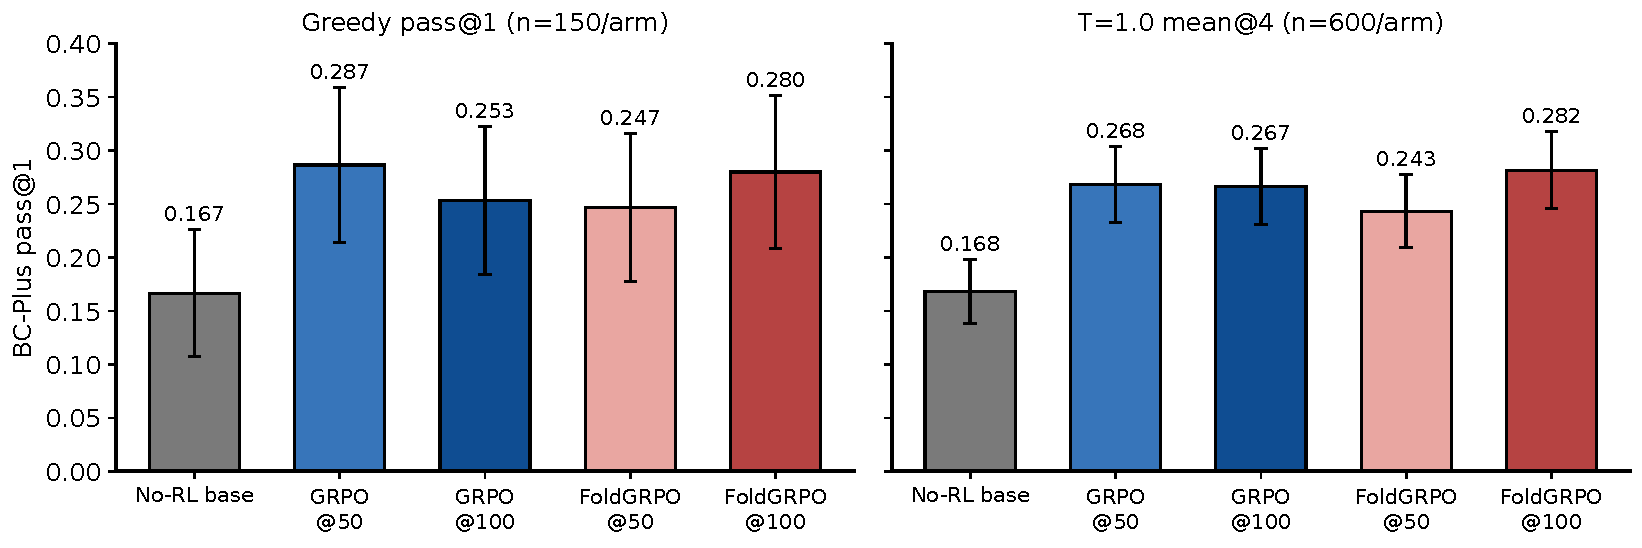
\includegraphics[width=0.9\linewidth]{figures/fig1_scores_by_arm.pdf}
\caption{\bcplus{} pass@1 by arm at both operating points. Error bars are 95\% binomial CIs
(greedy: $n{=}150$ items; $T{=}1.0$ tier: $n{=}600$ graded samples). Only uncontaminated cells
are shown (\cref{sec:contamination}).}
\label{fig:scores}
\end{figure}

\paragraph{Training dynamics.} \Cref{fig:training} shows per-step training reward with the
10-step-cadence validation overlay, and policy entropy. Both objectives collapse entropy to
$\approx 0.07$ within the first steps. An infrastructure outage zeroed rewards late in the
\grpo{} run; the tail was re-run from the step-90 checkpoint, leaving two genuine zero-reward
no-op steps (zero advantage implies zero gradient), so \grpo{} trained 98 effective steps of
100. The \foldgrpo{} run was clean.

\begin{figure}[t]
\centering
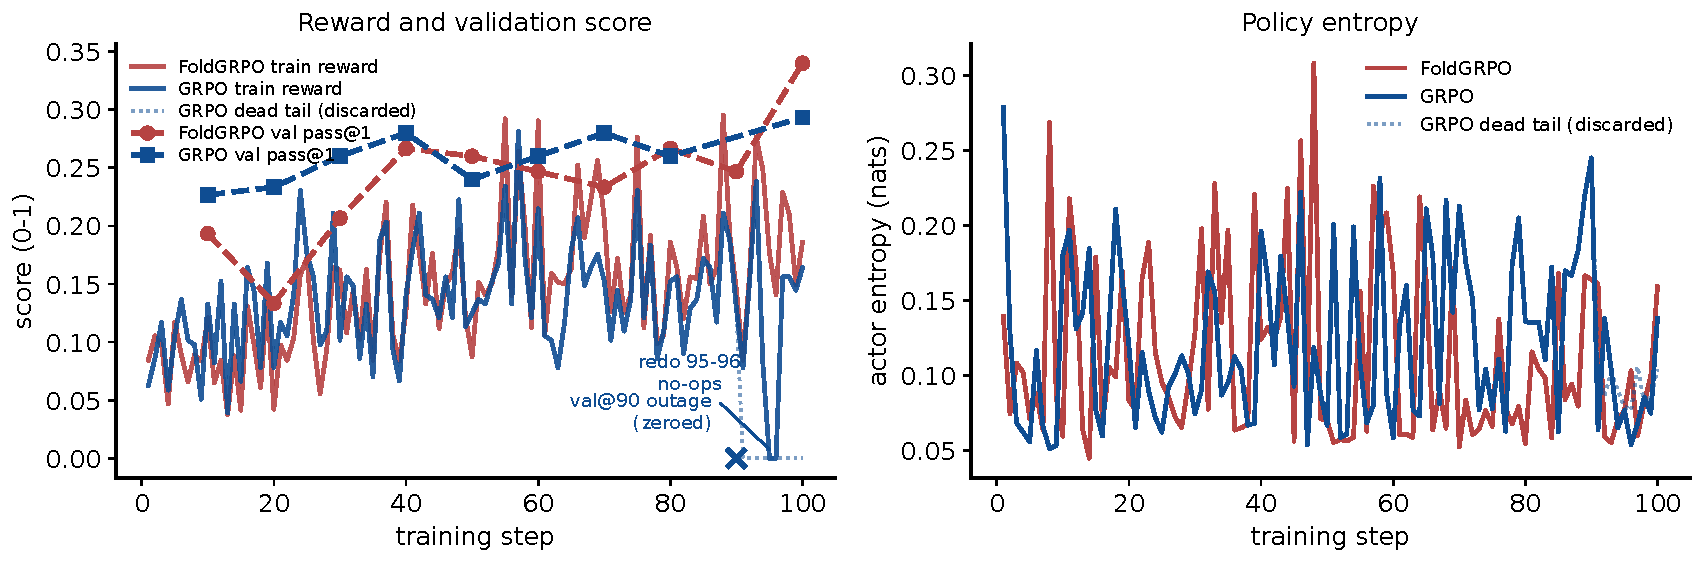
\includegraphics[width=\linewidth]{figures/fig2_training_curves.pdf}
\caption{Training curves for both RL arms: mean training reward with greedy validation score
overlaid every 10 steps (left) and policy entropy (right), parsed from the training logs (last
occurrence per step; the two \grpo{} no-op steps are marked).}
\label{fig:training}
\end{figure}
